\documentclass[12pt]{article}

%%%%%%%%%%%%%%%%%%%%%%%%%%%%%%%%%%%%%%%%%
% Lachaise Assignment
% Structure Specification File
% Version 1.0 (26/6/2018)
%
% This template originates from:
% http://www.LaTeXTemplates.com
%
% Authors:
% Marion Lachaise & François Févotte
% Vel (vel@LaTeXTemplates.com)
%
% License:
% CC BY-NC-SA 3.0 (http://creativecommons.org/licenses/by-nc-sa/3.0/)
% 
%%%%%%%%%%%%%%%%%%%%%%%%%%%%%%%%%%%%%%%%%

%----------------------------------------------------------------------------------------
%	PACKAGES AND OTHER DOCUMENT CONFIGURATIONS
%----------------------------------------------------------------------------------------

\usepackage{amsmath,amsfonts,stmaryrd,amssymb} % Math packages

\usepackage{enumerate} % Custom item numbers for enumerations

\usepackage[ruled]{algorithm2e} % Algorithms

\usepackage[framemethod=tikz]{mdframed} % Allows defining custom boxed/framed environments

\usepackage{listings} % File listings, with syntax highlighting
\lstset{
	basicstyle=\ttfamily, % Typeset listings in monospace font
}

%----------------------------------------------------------------------------------------
%	DOCUMENT MARGINS
%----------------------------------------------------------------------------------------

\usepackage{geometry} % Required for adjusting page dimensions and margins

\geometry{
	paper=a4paper, % Paper size, change to letterpaper for US letter size
	top=2.5cm, % Top margin
	bottom=3cm, % Bottom margin
	left=2.5cm, % Left margin
	right=2.5cm, % Right margin
	headheight=14pt, % Header height
	footskip=1.5cm, % Space from the bottom margin to the baseline of the footer
	headsep=1.2cm, % Space from the top margin to the baseline of the header
	%showframe, % Uncomment to show how the type block is set on the page
}

%----------------------------------------------------------------------------------------
%	FONTS
%----------------------------------------------------------------------------------------

\usepackage[utf8]{inputenc} % Required for inputting international characters
\usepackage[T1]{fontenc} % Output font encoding for international characters

\usepackage{XCharter} % Use the XCharter fonts

%----------------------------------------------------------------------------------------
%	COMMAND LINE ENVIRONMENT
%----------------------------------------------------------------------------------------

% Usage:
% \begin{commandline}
%	\begin{verbatim}
%		$ ls
%		
%		Applications	Desktop	...
%	\end{verbatim}
% \end{commandline}

\mdfdefinestyle{commandline}{
	leftmargin=10pt,
	rightmargin=10pt,
	innerleftmargin=15pt,
	middlelinecolor=black!50!white,
	middlelinewidth=2pt,
	frametitlerule=false,
	backgroundcolor=black!5!white,
	frametitle={Command Line},
	frametitlefont={\normalfont\sffamily\color{white}\hspace{-1em}},
	frametitlebackgroundcolor=black!50!white,
	nobreak,
}

% Define a custom environment for command-line snapshots
\newenvironment{commandline}{
	\medskip
	\begin{mdframed}[style=commandline]
}{
	\end{mdframed}
	\medskip
}

%----------------------------------------------------------------------------------------
%	FILE CONTENTS ENVIRONMENT
%----------------------------------------------------------------------------------------

% Usage:
% \begin{file}[optional filename, defaults to "File"]
%	File contents, for example, with a listings environment
% \end{file}

\mdfdefinestyle{file}{
	innertopmargin=1.6\baselineskip,
	innerbottommargin=0.8\baselineskip,
	topline=false, bottomline=false,
	leftline=false, rightline=false,
	leftmargin=2cm,
	rightmargin=2cm,
	singleextra={%
		\draw[fill=black!10!white](P)++(0,-1.2em)rectangle(P-|O);
		\node[anchor=north west]
		at(P-|O){\ttfamily\mdfilename};
		%
		\def\l{3em}
		\draw(O-|P)++(-\l,0)--++(\l,\l)--(P)--(P-|O)--(O)--cycle;
		\draw(O-|P)++(-\l,0)--++(0,\l)--++(\l,0);
	},
	nobreak,
}

% Define a custom environment for file contents
\newenvironment{file}[1][File]{ % Set the default filename to "File"
	\medskip
	\newcommand{\mdfilename}{#1}
	\begin{mdframed}[style=file]
}{
	\end{mdframed}
	\medskip
}

%----------------------------------------------------------------------------------------
%	NUMBERED QUESTIONS ENVIRONMENT
%----------------------------------------------------------------------------------------

% Usage:
% \begin{question}[optional title]
%	Question contents
% \end{question}

\mdfdefinestyle{question}{
	innertopmargin=1.2\baselineskip,
	innerbottommargin=0.8\baselineskip,
	roundcorner=5pt,
	nobreak,
	singleextra={%
		\draw(P-|O)node[xshift=1em,anchor=west,fill=white,draw,rounded corners=5pt]{%
		Question \theQuestion\questionTitle};
	},
}

\newcounter{Question} % Stores the current question number that gets iterated with each new question

% Define a custom environment for numbered questions
\newenvironment{question}[1][\unskip]{
	\bigskip
	\stepcounter{Question}
	\newcommand{\questionTitle}{~#1}
	\begin{mdframed}[style=question]
}{
	\end{mdframed}
	\medskip
}

%----------------------------------------------------------------------------------------
%	WARNING TEXT ENVIRONMENT
%----------------------------------------------------------------------------------------

% Usage:
% \begin{warn}[optional title, defaults to "Warning:"]
%	Contents
% \end{warn}

\mdfdefinestyle{warning}{
	topline=false, bottomline=false,
	leftline=false, rightline=false,
	nobreak,
	singleextra={%
		\draw(P-|O)++(-0.5em,0)node(tmp1){};
		\draw(P-|O)++(0.5em,0)node(tmp2){};
		\fill[black,rotate around={45:(P-|O)}](tmp1)rectangle(tmp2);
		\node at(P-|O){\color{white}\scriptsize\bf !};
		\draw[very thick](P-|O)++(0,-1em)--(O);%--(O-|P);
	}
}

% Define a custom environment for warning text
\newenvironment{warn}[1][Warning:]{ % Set the default warning to "Warning:"
	\medskip
	\begin{mdframed}[style=warning]
		\noindent{\textbf{#1}}
}{
	\end{mdframed}
}

%----------------------------------------------------------------------------------------
%	INFORMATION ENVIRONMENT
%----------------------------------------------------------------------------------------

% Usage:
% \begin{info}[optional title, defaults to "Info:"]
% 	contents
% 	\end{info}

\mdfdefinestyle{info}{%
	topline=false, bottomline=false,
	leftline=false, rightline=false,
	nobreak,
	singleextra={%
		\fill[black](P-|O)circle[radius=0.4em];
		\node at(P-|O){\color{white}\scriptsize\bf i};
		\draw[very thick](P-|O)++(0,-0.8em)--(O);%--(O-|P);
	}
}

% Define a custom environment for information
\newenvironment{info}[1][Info:]{ % Set the default title to "Info:"
	\medskip
	\begin{mdframed}[style=info]
		\noindent{\textbf{#1}}
}{
	\end{mdframed}
}

\title{VE527: Assignment \#3} % Title of the assignment
\author{Name: Chang Meng\\Student ID:\@\texttt{118370910019}}
\date{\today}

\begin{document}

    \maketitle

    \section{(8\%) Static Timing Analysis: Basics}

    Which of the following statements about static timing analysis are
    correct?

    \begin{enumerate}[a)]
        \item All nodes on the longest delay path from source to sink will
            have the worst case slack value.
        \item To find the worst paths in decreasing delay order, we can use
            an algorithm that is similar to maze routing by storing the
            partial paths in a heap, where the item with the most positive
            slack is alwagys on the top.
        \item To find the longest path, we can simply enumerate ALL the source-
            to-sink paths in the delay graph. This is efficient enough since
            the paths will not be too many.
        \item A positive slact at a node means the node does not meet timing
            requirement, so it is always bad to see positive slack.
        \item Negative slack is always bad and indicates a timing problem.
        \item We may get a false longest path in static timing analysis because
            we ignore the logic of the circuit.
    \end{enumerate}

    \noindent
    Answer:
    a), e) and f) are correct.

    \section{(45\%) Static Timing Analysis}

    Consider the small logic network shown below. There are 6 primary inputs (PIs)
    labeled A, B, C, D, E, F. There is 1 primary output (PO) Z. There are 11 logic
    gates. There are 10 internal wires that represent gate outputs/inputs, labeled:
    w1, w2, ..., w10. The gate delay for each inverter is 2. The gate delay for each
    NAND2 is 3. Ignore delay for the wires. This logic operates on a clock with a
    cycle time = 15.

    \begin{center}
        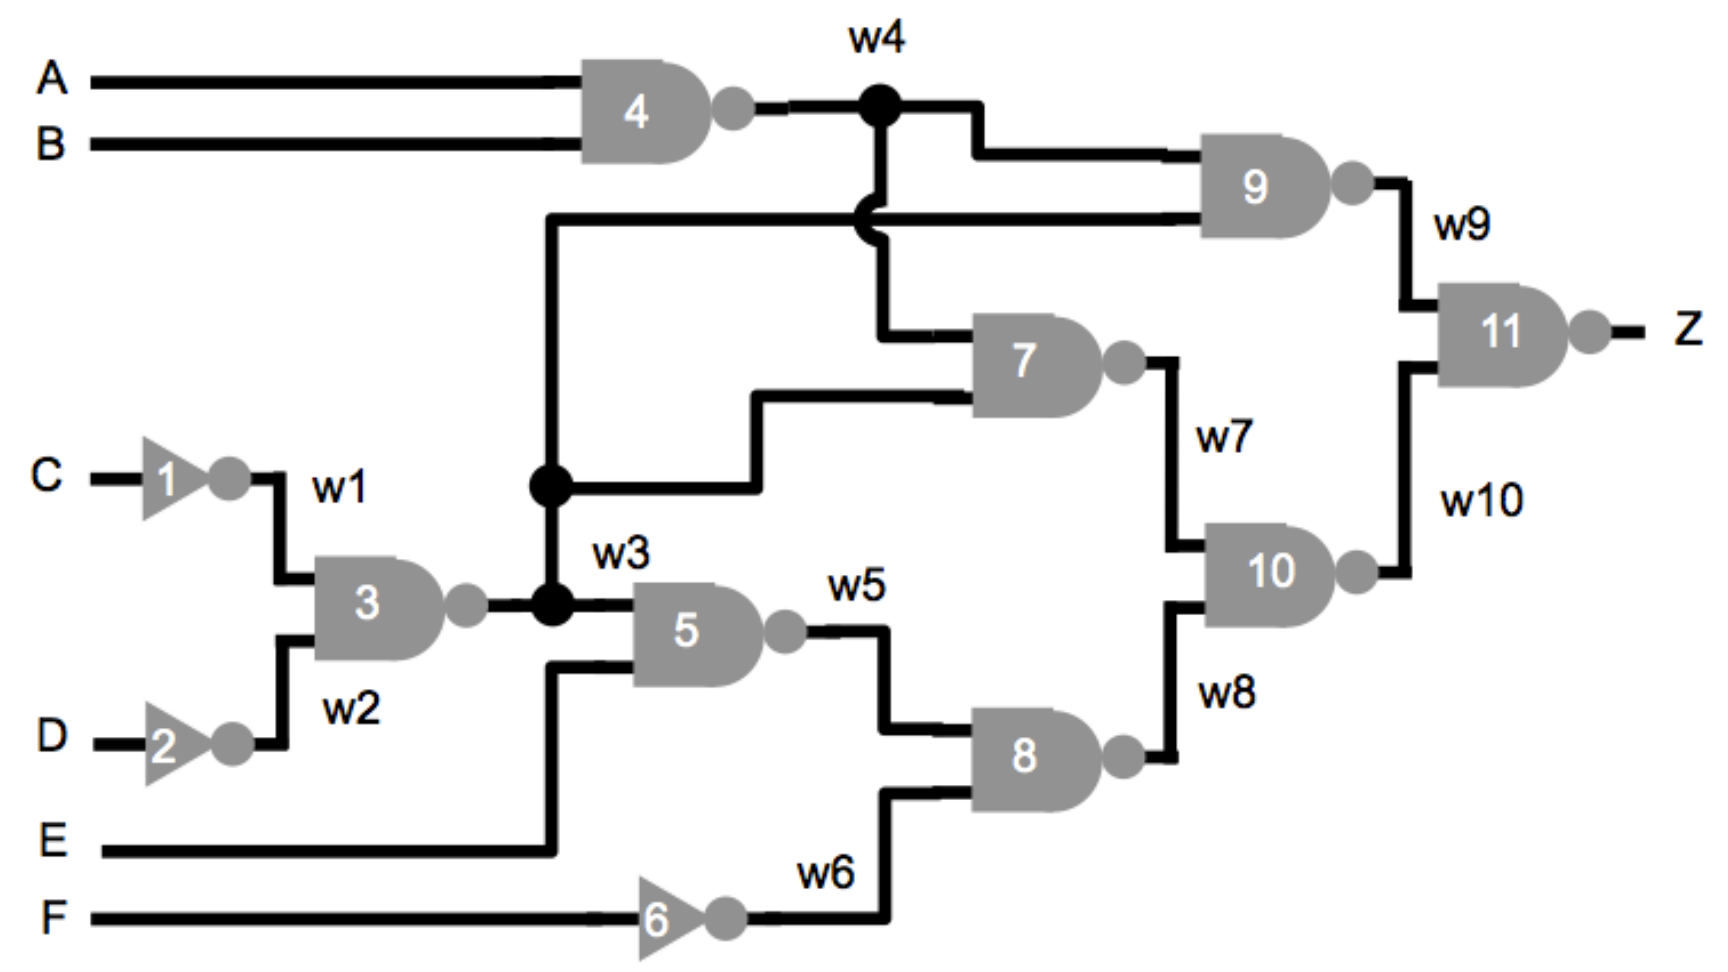
\includegraphics[width = 5.60in, height = 3.20in]{figure1.png}
    \end{center}

    \noindent
    Draw the Delay Graph for this logic network, including one source and on sink node,
    and appropriate edges representing all the delays. Then, calculate the arrival
    time (AT), the required arrival time (RAT), and the slack for each node in the
    graph. Is there a timing violation? Report a longest path in the graph.

    \vspace{12pt}

    \noindent
    Answer:

    \noindent
    The Delay Graph is shown below:

    \begin{center}
        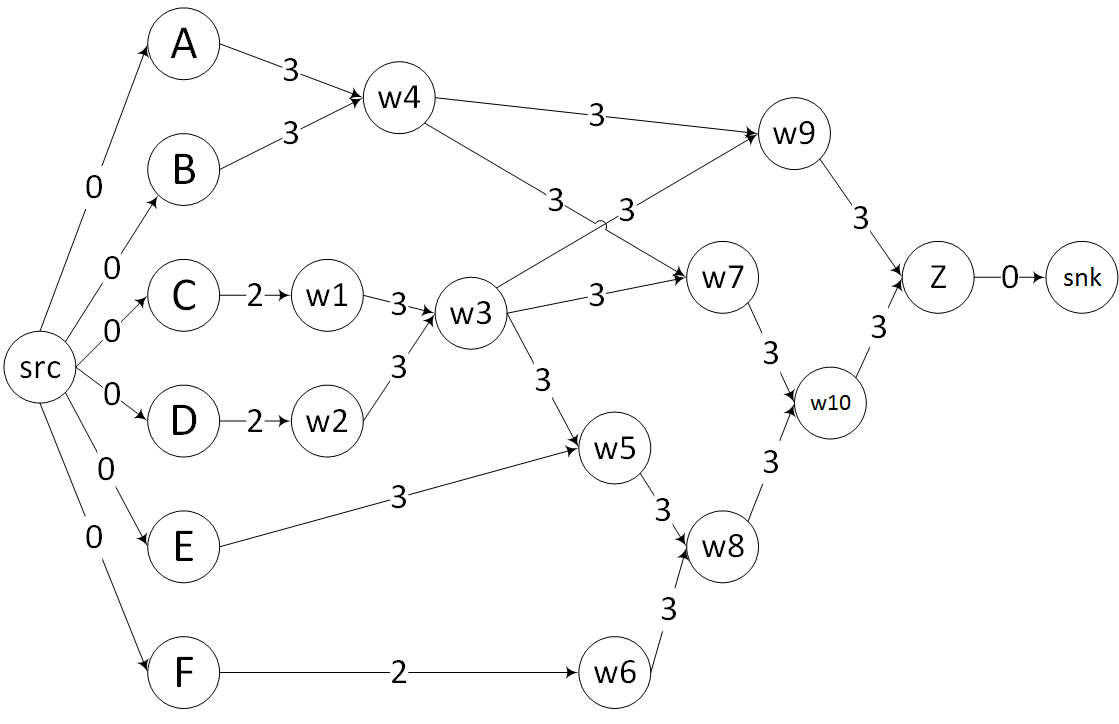
\includegraphics[width = 5.60in, height = 3.20in]{figure2.png}
    \end{center}

    The calculation process of AT is demonstrated in the following chart:

    \begin{center}
    \begin{tabular}{|c|c|c|}
        \hline
        node & predecessors & AT \\
        \hline
        src & $\verb|\|$ & $0$ \\
        \hline
        A & src & $0$ \\
        \hline
        B & src & $0$ \\
        \hline
        C & src & $0$ \\
        \hline
        D & src & $0$ \\
        \hline
        E & src & $0$ \\
        \hline
        F & src & $0$ \\
        \hline
        w1 & C & $AT(C)+2=2$ \\
        \hline
        w2 & D & $AT(D)+2=2$ \\
        \hline
        w3 & w1, w2 & $max\{AT(w1)+3,AT(w2)+3\}=5$ \\
        \hline
        w4 & A, B & $max\{AT(A)+3,AT(B)+3\}=3$ \\
        \hline
        w5 & w3, E & $max\{AT(w3)+3,AT(E)+3\}=8$ \\
        \hline
        w6 & F & $AT(F)+2=2$ \\
        \hline
        w7 & w3, w4 & $max\{AT(w3)+3,AT(w4)+3\}=8$ \\
        \hline
        w8 & w5, w6 & $max\{AT(w5)+3,AT(w6)+3\}=11$ \\
        \hline
        w9 & w3, w4 & $max\{AT(w3)+3,AT(w4)+3\}=8$ \\
        \hline
        w10 & w7, w8 & $max\{AT(w7)+3,AT(w8)+3\}=14$ \\
        \hline
        Z & w9, w10 & $max\{AT(w9)+3,AT(w10)+3\}=17$ \\
        \hline
        snk & Z & $17$ \\
        \hline
    \end{tabular}
    \end{center}

    \vspace{12pt}

    The calculation process of RAT is demonstrated in the following chart:

    \begin{tabular}{|c|c|c|}
        \hline
        node & successors & RAT \\
        \hline
        snk & $\verb|\|$ & 15 \\
        \hline
        Z & snk & 15 \\
        \hline
        w10 & Z & $RAT(Z)-3=12$ \\
        \hline
        w9 & Z & $RAT(Z)-3=12$ \\
        \hline
        w8 & w10 & $RAT(w10)-3=9$ \\
        \hline
        w7 & w10 & $RAT(w10)-3=9$ \\
        \hline
        w6 & w8 & $RAT(w8)-3=6$ \\
        \hline
        w5 & w8 & $RAT(w8)-3=6$ \\
        \hline
        w4 & w7, w9 & $min\{RAT(w7)-3,RAT(w9)-3\}=6$ \\
        \hline
        w3 & w5, w7, w9 & $min\{RAT(w5)-3,RAT(w7)-3,RAT(w9)-3\}=3$ \\
        \hline
        w2 & w3 & $RAT(w3)-3=0$ \\
        \hline
        w1 & w3 & $RAT(w3)-3=0$ \\
        \hline
        A & w4 & $RAT(w4)-3=3$ \\
        \hline
        B & w4 & $RAT(w4)-3=3$ \\
        \hline
        C & w1 & $RAT(w1)-2=-2$ \\
        \hline
        D & w2 & $RAT(w2)-2=-2$ \\
        \hline
        E & w5 & $RAT(w5)-3=3$ \\
        \hline
        F & w6 & $RAT(w6)-2=4$ \\
        \hline
        src & A, B, C, D, E, F, G & $min\{RAT(A),RAT(B),...,RAT(F)\}=-2$ \\
        \hline
    \end{tabular}

    \vspace{12pt}

    The calculation process of slack is demonstrated in the following chart:

    \begin{center}
    \begin{tabular}{|c|c|c|c|}
        \hline
        node & AT & RAT & slack \\
        \hline
        src & 0 & -2 & -2 \\
        \hline
        A & 0 & 3 & 3 \\
        \hline
        B & 0 & 3 & 3 \\
        \hline
        C & 0 & -2 & -2 \\
        \hline
        D & 0 & -2 & -2 \\
        \hline
        E & 0 & 3 & 3 \\
        \hline
        F & 0 & 4 & 4 \\
        \hline
        w1 & 2 & 0 & -2 \\
        \hline
        w2 & 2 & 0 & -2 \\
        \hline
        w3 & 5 & 3 & -2 \\
        \hline
        w4 & 3 & 6 & 3 \\
        \hline
        w5 & 8 & 6 & -2 \\
        \hline
        w6 & 2 & 6 & 4 \\
        \hline
        w7 & 8 & 9 & 1 \\
        \hline
        w8 & 11 & 9 & -2 \\
        \hline
        w9 & 8 & 12 & 4 \\
        \hline
        w10 & 14 & 12 & -2 \\
        \hline
        Z & 17 & 15 & -2 \\
        \hline
        snk & 17 & 15 & -2 \\
        \hline
    \end{tabular}
    \end{center}

    For nodes src, C, D, w1, w2, w3, w5, w8, w10, Z and snk, their slacks are negative,
    so there exists a timing violation.

    Since all nodes on longest path have samve worst slack value, so one of the longest
    paths is:

    src->C->w1->w3->w5->w8->w10->Z->snk

    \section{(4\%) Elmore Deley Analysis: Basics}
    Which of the following statements about Elmore delay analysis are correct?
    \begin{enumerate}[a)]
        \item According to Elmore delay, the delay between the root node and a leaf node
            in an RC tree equals to the root node resistance times the downstream capacitance.
        \item Elmore delay is the most presice and accurate measure of the electrical delay
            through an RC network. Thus it is very popular.
        \item The capacitance of a metal wire is proportional to its width and its length.
        \item The resistance of a metal wire segment is proportional to its width and inversely
            proportional to its length.
        \item In a multi-point net, the Elmore delay from the root to each leaf is the same.
    \end{enumerate}

    \noindent
    Answer:

    \noindent
    c) is correct.

    \section{(43\%) Elmore Delay Calculation}
    Consider a chip-level long interconnect wire shown in the figure below. The wire is a
    4-point net: gate a drives the net; gates b, c, and d are driven by the net. The wire
    decomposes into 6 separate metal segments, with 3 internal nodes labels 1, 2 and 3 in
    the figure. The length of each wire is labeled next to each wire.

    \begin{center}
        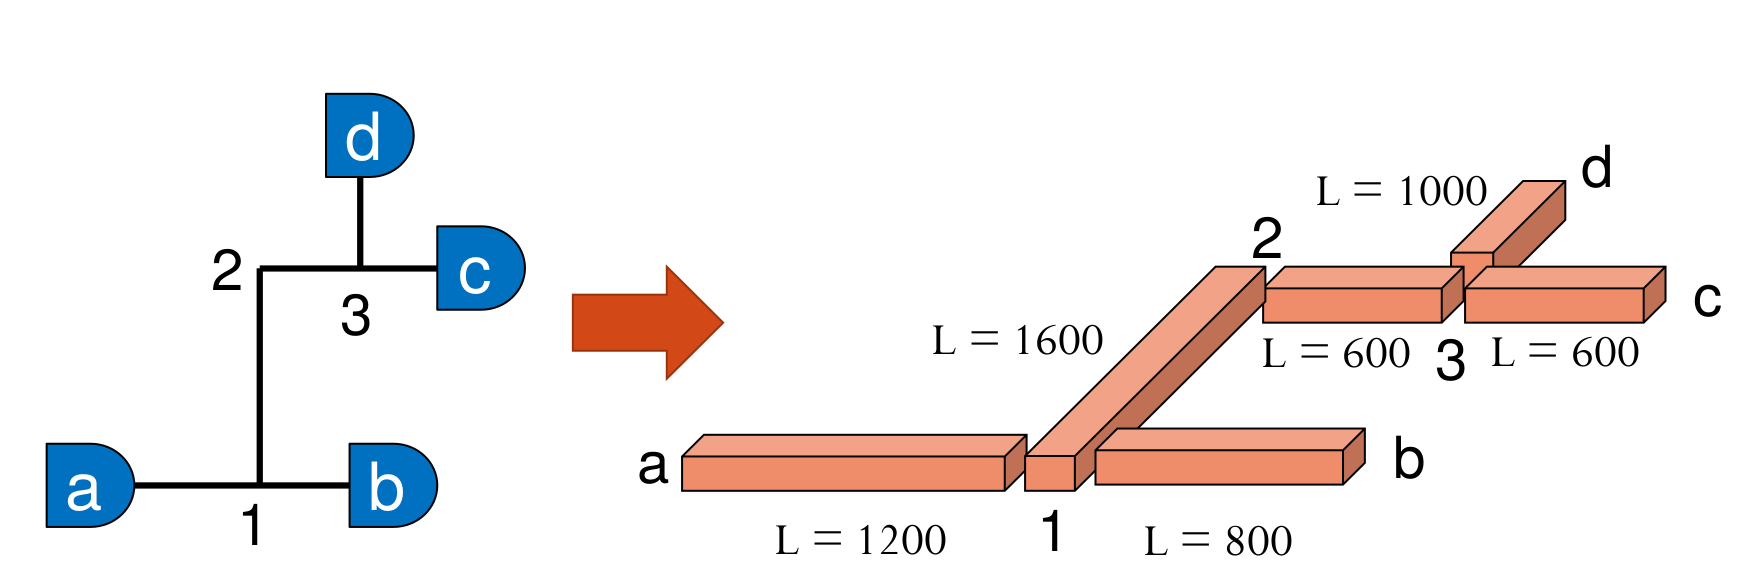
\includegraphics[width = 6.60in, height = 2.00in]{figure3.png}
    \end{center}

    \noindent
    The table below further gives the detailed dimension of each wire segment (including the
    width).

    \begin{center}
        \begin{tabular}{|c|c|c|}
            \hline
            Segment & Length L & Width W \\
            \hline
            a-1 & 1200 & 1 \\
            \hline
            1-b & 800 & 0.5 \\
            \hline
            1-2 & 1600 & 1 \\
            \hline
            2-3 & 600 & 0.5 \\
            \hline
            3-c & 600 & 0.5 \\
            \hline
            3-d & 1000 & 0.5 \\
            \hline
        \end{tabular}
    \end{center}

    \noindent
    We further assume the following electrical parameters:
    \begin{itemize}
        \item Resistance of driver gate a: $500$
        \item Capacitance of driver gates b, c, d: $1\times 10^{-7}$
        \item Resistance const $r=\frac{\rho}{H}=0.5$
        \item Capacitance const $c=\frac{\epsilon}{d}=1\times 10^{-9}$
    \end{itemize}

    \noindent
    Don't worry about the units. Do the following:

    \begin{enumerate}[(a)]
    \item (25\%) Draw the RC tree model for this wire, including the effect from driver and
    driven gates.
    \item (18\%) Calculate the Elmore delay from the driver to each of the driven gates, i.e.,
    the delay from a to b, the delay from a to c, and the delay from a to d.
    \end{enumerate}

    \noindent
    Answer:

    \noindent
    (a) Since we have:
    \[R=\frac{rL}{W}\]
    \[C=cWL\]

    The capacitance and resistance of each segments are derived in the following table:
    \begin{center}
        \begin{tabular}{|c|c|c|c|c|}
            \hline
            Segment & Length L & Width W & resistance & capacitance \\
            \hline
            a-1 & 1200 & 1 & 600 & $1.2\times 10^{-6}$ \\
            \hline
            1-b & 800 & 0.5 & 800 & $4\times 10^{-7}$ \\
            \hline
            1-2 & 1600 & 1 & 800 & $1.6\times 10^{-6}$ \\
            \hline
            2-3 & 600 & 0.5 & 600 & $3\times 10^{-7}$ \\
            \hline
            3-c & 600 & 0.5 & 600 & $3\times 10^{-7}$ \\
            \hline
            3-d & 1000 & 0.5 & 1000 & $5\times 10^{-7}$ \\
            \hline
        \end{tabular}
    \end{center}

    The equivalent capacitance on each nodes is:
    \begin{center}
        \begin{tabular}{|c|c|c|c|c|}
            \hline
            node & where the capacitance comes from & equivalent capacitance \\
            \hline
            a & segment a-1 & $1.2\times 10^{-6}/2=6\times 10^{-7}$ \\
            \hline
            1 & segment a-1, 1-2 and 1-b & $(1.2+1.6+0.4)\times 10^{-6}/2=1.6\times 10^{-6}$\\
            \hline
            2 & segment 1-2 and 2-3 & $(1.6+0.3)\times 10^{-7}/2=9.5\times 10^{-7}$ \\
            \hline
            3 & segment 2-3, 3-d and 3-c & $(3+3+5)\times 10^{-7}/2=5.5\times 10^{-7}$ \\
            \hline
            b & segment 1-b and gate b & $(4/2+1)\times 10^{-7}=3\times 10^{-7}$ \\
            \hline
            c & segment 3-c and gate c & $(3/2+1)\times 10^{-7}=2.5\times 10^{-7}$ \\
            \hline
            d & segment 3-d and gate d & $(5/2+1)\times 10^{-7}=3.5\times 10^{-7}$ \\
            \hline
        \end{tabular}
    \end{center}

    The RC tree model for this wire is shown below:

    \begin{center}
        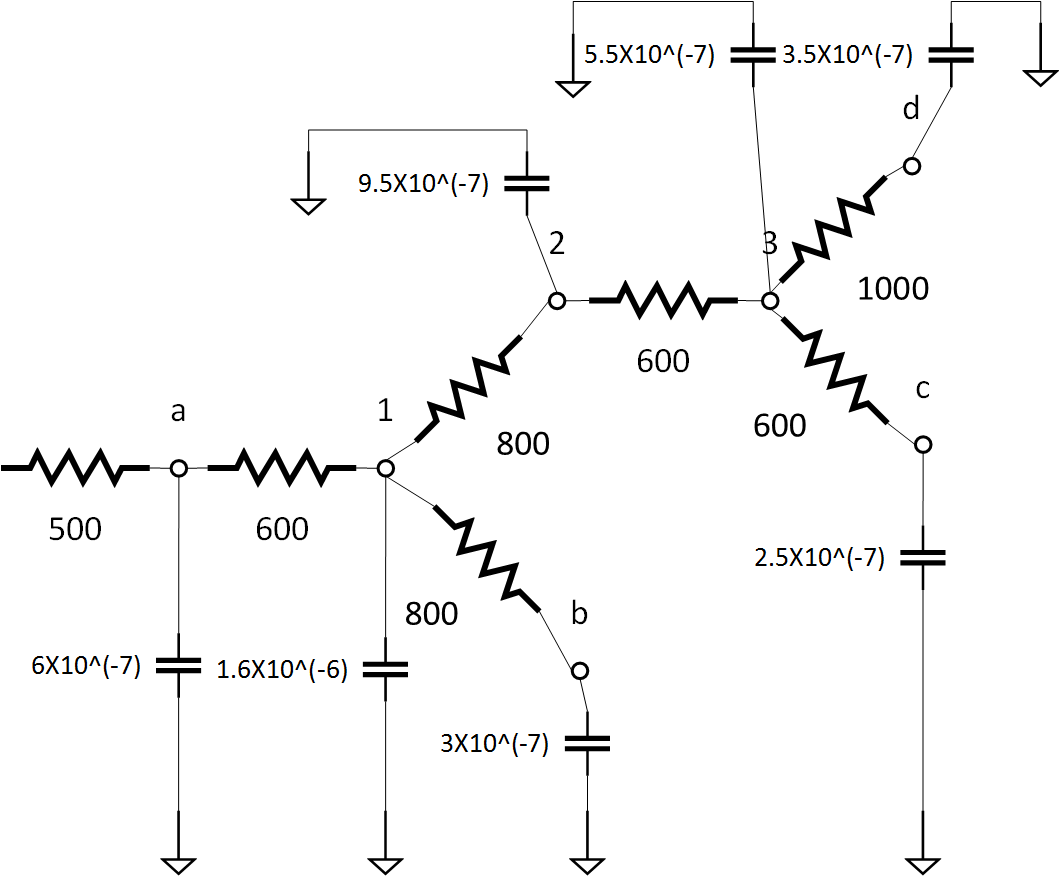
\includegraphics[width = 6.50in, height = 4.30in]{figure4.png}
    \end{center}

    \noindent 
    (b)\\
    The Elmore delay from a to b is:
    \[
        \begin{split}
            & \tau_{ab}= \\
            & 800\times 3\times 10^{-7} \\ 
            & + 600 \times (16+3+9.5+5.5+3.5+2.5)\times 10^{-7} \\
            & + 500 \times (6+16+3+9.5+5.5+3.5+2.5)\times 10^{-7} \\
            & = 4.94 \times 10^{-3}
        \end{split}
    \]

    The Elmore delay from a to c is:
    \[
        \begin{split}
            & \tau_{ac}= \\
            & 600\times 2.5\times 10^{-7} \\ 
            & + 600\times (5.5+3.5+2.5)\times 10^{-7} \\
            & + 800 \times (9.5+5.5+3.5+2.5)\times 10^{-7} \\
            & + 600 \times (16+3+9.5+5.5+3.5+2.5)\times 10^{-7} \\
            & + 500 \times (6+16+3+9.5+5.5+3.5+2.5)\times 10^{-7} \\
            & = 7.22 \times 10^{-3}
        \end{split}
    \]

    The Elmore delay from a to d is:
    \[
        \begin{split}
            & \tau_{ad}= \\
            & 1000\times 3.5\times 10^{-7} \\ 
            & + 600\times (5.5+3.5+2.5)\times 10^{-7} \\
            & + 800 \times (9.5+5.5+3.5+2.5)\times 10^{-7} \\
            & + 600 \times (16+3+9.5+5.5+3.5+2.5)\times 10^{-7} \\
            & + 500 \times (6+16+3+9.5+5.5+3.5+2.5)\times 10^{-7} \\
            & = 7.42 \times 10^{-3}
        \end{split}
    \]
\end{document}
